\chapter{A LINGUAGEM PARA ESPECIFICAÇÃO DE CONTRATOS NEOIDL}
\vspace{-6mm}
%

\section{NeoIDL}

 

\subsection{Objetivos}
\vspace{-6mm}

\subsection{Histórico}
\vspace{-6mm}

\subsection{Arquitetura do framework}
\vspace{-6mm}


\subsection{Avaliações}
\vspace{-6mm}

\subsubsection{Expressividade}
\vspace{-6mm}

Nesta subseção falar da avaliação feita nos contratos do exército.

\subsubsection{Potencial de reuso}

Complementar a avaliação de expressividade com o potencial de reuso.

 
\subsection{Extensão da linguagem}

Influência de Eiffel, JML e Spec\#

Eiffel assertions are Boolean expressions, with a few extensions such as the old
notation. Since the whole power of Boolean expressions is available, they may
include function calls. Because the full power of the language is available to
write these functions, the conditions they express can be quite sophisticated.
\cite{meyer1992applying}

 
 
\section{Proposta: Serviços com Desing-by-Contract}
\vspace{-6mm}

Os benefícios esperados pela adoção da arquitetura orientada a serviços
somente serão auferidos com a concepção adequada de cada serviço. 
Por essa razão, é necessário planejar o projeto dos serviços criteriosamente
antes de lançar mão do desenvolvimento, com preocupação especial em garantir
um nível aceitável de estabilidade aos consumidores de cada serviço.
Nessa etapa do projeto de desenho da solução, a especificação do contrato do
serviço (Web API) exerce uma função fundamental. 

Na sociedade civil, contratos são meios de se formalizar acordo entre partes a
fim de definir os direitos e deveres de cada parte e buscar atingir o
objetivo esperado dentro de determinadas regras. Cada parte espera que as outras
cumpram com suas obrigações.
Por outro lado, sabe-se que o descumprimeto das obrigações costuma implicar de
penalizações até o desfazimento do contrato. 

Contratos entre serviços Web seguem em uma linha análoga. O desenho das
capacidades (operações) e dos dados das mensagens correspondem aos
termos do contrato no sentido do que o consumidor deve esperar do serviço
provedor. Porém identificou-se, após ampla pesquisa realizada sobre o tema, que
as linguagens disponíves para especificação de contratos atingem apenas esse
nível de garantias. No contexto de webservices em REST, conforme descrito na
seção \ref{secaoREST}, há ainda a ausência de padrão para especificação
contratos, tal como ocorre com o WSDL adotado em SOAP.

A proposta deste trabalho é extender os níveis de garantias, de modo a promover
um patamar adicional com obrigações mutuas entre os serviços (consumidor e
provedor). Isso se dá para adoção do conceito de Design-by-Contract (debatido
na seção \ref{Design-by-Contract}) em que a execução da
capacidade do serviço garantirá a execução, desde que satisfeitas as condições
prévias. O detalhamento do processo é exposto nas seções que se seguem.

\vspace{-6mm}

\subsection{Modelo de operação}
\vspace{-6mm}

As garantias para execução dos serviços são estabelecidas em duas etapas: pré- e
pós-condições. Nas pré-condições o provedor do serviço estabelece os requisitos
para que o serviço possa ser executado. A etapa de pós-condições tem o papel de
validar se a mensagem de retorno do serviço possui resultados válidos.

O diagrama da Figura \ref{FigServiceDbC} descreve como ocorre a operação das
pré- e pós-condições. O processo se inicia com a chamada à capacidade do serviço e a
identificação da existência de uma pré-condição. Caso tenham sido estabelecidas 
pré-condições, essas são avaliadas. Caso alguma delas não tenham sido
satisfeitas, o serviço principal não é processado e o provedor do serviço
retornar o código de falha definido no contrato correspondente.


\begin{figure}[!htb]
\centering
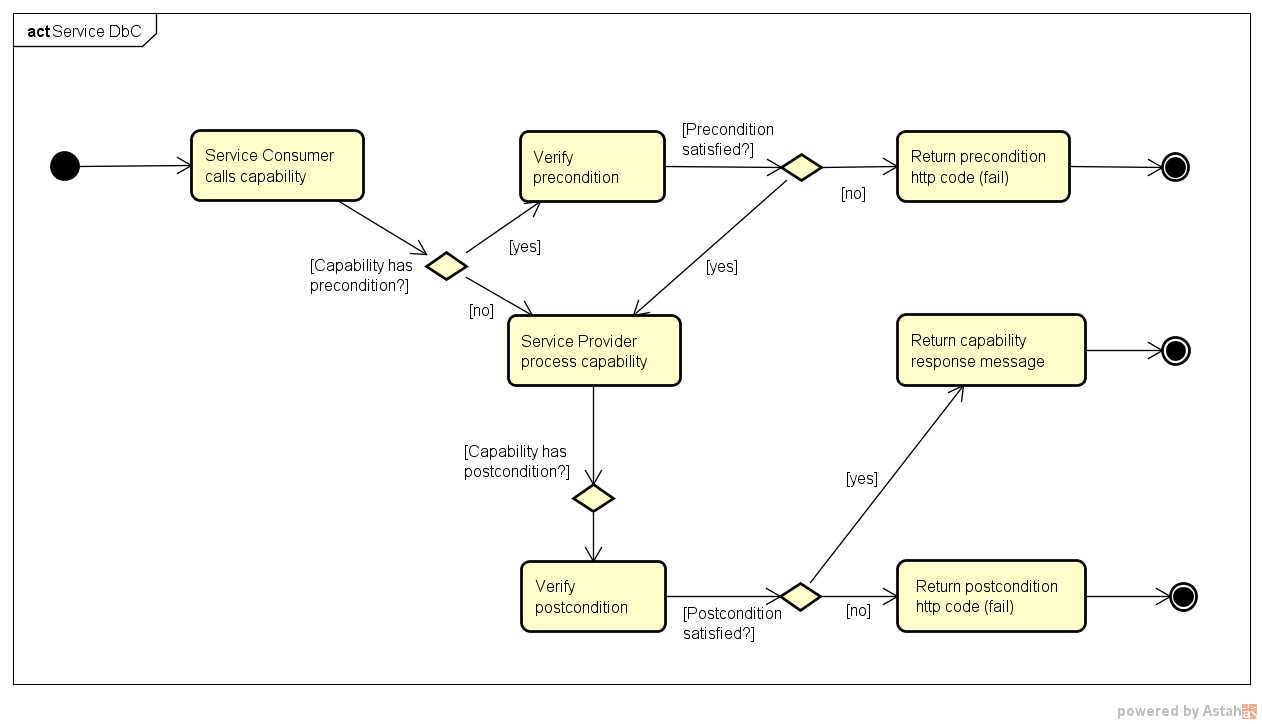
\includegraphics[width=\textwidth,trim = 0mm 5mm 0mm 0mm,clip]{ServiceDbC.png}
\caption{Digrama de atividades com verificação de pré e pós condições}
\label{FigServiceDbC}
\end{figure}

Caso tenham sido definidas pós-condições, essas são acionadas após o
processamento da capacidade, porém antes do retorno ao consumidor do serviço.
Assim, conforme Figura \ref{FigServiceDbC}, visando não entregar ao cliente uma
mensagem ou situação incoerente, as pós-condições são validadas. Caso todas as
pós-condições tenham sido satisfeitas, a mensagem de retorno é encaminhada ao
cliente. Caso contrário, será retornado o código de falha.


\vspace{-6mm}


\subsubsection{Verificação das pré-condições}
\vspace{-6mm}

As pré-condições podem ser do tipo baseado nos parâmetros da requisição ou do
tipo baseado na chamada a outro serviço. Denominamos, para o contexto desta
dissertação, de básica a pré-condição baseada apenas nos parâmetros da
requisição (atributos da chamada ao serviço). Nessa validação é direta,
comparando os valores passados com os valores admitidos. 

No caso das pré-condições baseadas em serviços, é realizada chamada a outro
serviço para verificar se uma determinada condição é satisfeita. Este modo de
funcionamento, que se assemelha a uma composição de serviço, é mais versátil, pois permite
validações de condições complexas sem que a lógica associada seja conhecida pelo
cliente. Assim, os contratos que estabelecem esse tipo de
pré-condição se mantem simples.

A Figura \ref{FigServicePrecondition} detalha as etapas de verificação de cada
pré-condição. Nota-se que a saída para as situações de desatendimento às
pré-condições, independentemente do tipo, é o mesmo. O objetivo desta abordagem
é simplificar o tratametno de exceção no consumidor.

\begin{figure}[!htb]
\centering
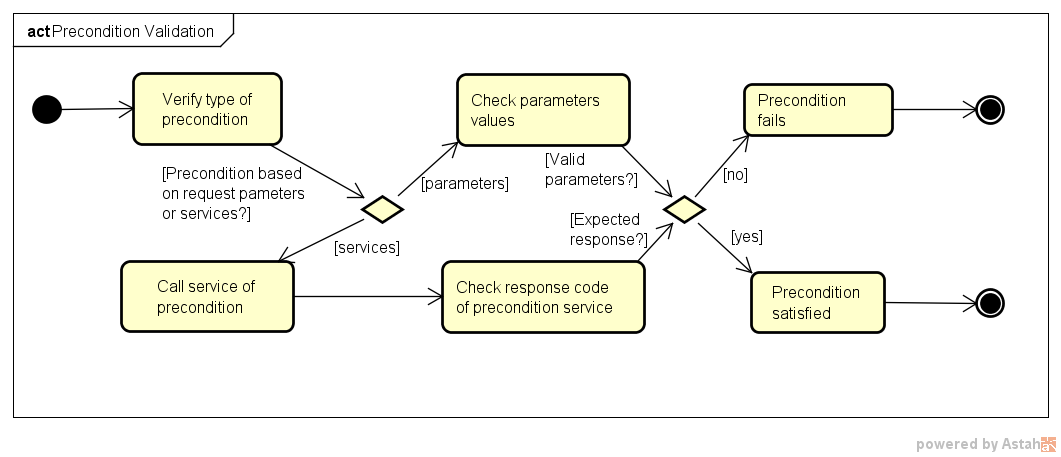
\includegraphics[width=\textwidth,trim = 0mm 5mm 0mm 0mm,clip]{PreconditionValidation.png}
\caption{Diagrama de atividades do processamento da pré-condição}
\label{FigServicePrecondition}
\end{figure}


\subsubsection{Verificação das pós-condições}
\vspace{-6mm}

\begin{figure}[!htb]
\centering
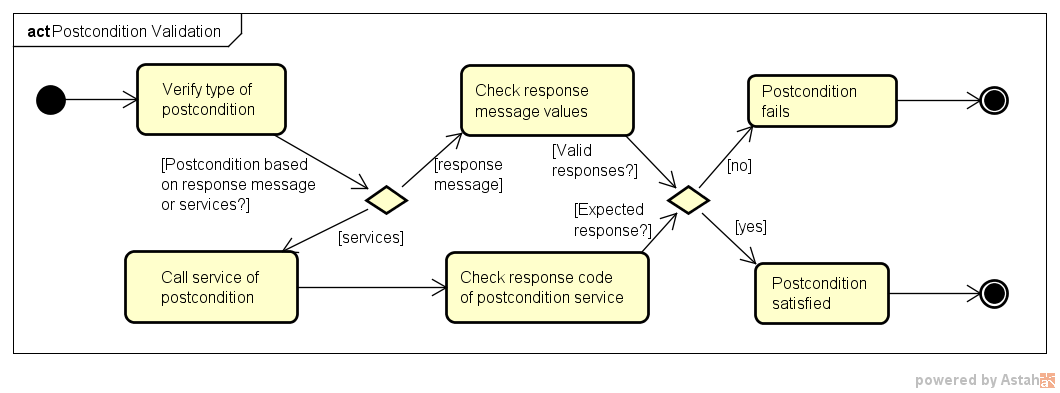
\includegraphics[width=\textwidth,trim = 0mm 5mm 0mm
0mm,clip]{PostconditionValidation.png} 
\vspace{-6mm}
\caption{Diagrama de atividades do processamento da pós-condição}
\label{FigServicePostcondition}
\end{figure}

A verificação das pós-condições acontece de modo muito similar a das
pré-condições. Há também os dois tipos, baseado em valores e em chamadas a
outros serviços. O diferencial está em que a validação dos valores passa a
ocorrer a partir dos valores contidos na mensagem de retorno. A Figura
\ref{FigServicePostcondition} descreve as etapas necessárias para validação de
cada pré-condição.

	

\section{Implementação de Design-by-Contract na NeoIDL}

\subsection{Pré-condição básica}

\begin{figure}[htb]
\begin{small}
\lstinputlisting[language=NeoIDL,firstnumber=1]{DBCsimple.neo}
\end{small}
\caption{Exemplo da notação DBC básica na \neoidl}
\label{lst:DBCService}
\end{figure}

\subsection{Pós-condição básica}

\ldots

\subsection{Pré-condição com chamada a serviço}

\ldots

\subsection{Pós-condição com chamada a serviço}

\ldots

\section{Estudo de caso}

\ldots

\subsection{Pluggin Twisted}

% Diagrama da estrutura do código gerado
